\appendix

\section{Implementation details}
\label{app: settings}
To ensure the robustness of tool calling, we implement TimeART based on Langchain, the api of all 21 tools are introduced in Appendix~\ref{app: tool}. Since our proposed training strategy does not involve reinforcement learning (RL), all stages can be organized as supervised fine-tuning (SFT). We adopt the LLaMA-Factory to achieve all the training stages, utilizing DeepSpeed ZeRO-3 for efficient training. The fine-tuning is performed in BF16 precision with FlashAttention-2 enabled to accelerate attention operations. We utilize LoRA, please refer to Table~\ref{tab:lora_hyperparams} for detailed configurations. The Training Curve is shown in Figure~\ref{fig: training curve}.


\begin{table}[!htbp]
    \centering
    \caption{Hyper-parameters and training time of fine-tuning the Qwen3 8B based on the TimeToolBench.}
    \label{tab:lora_hyperparams}
    \resizebox{1\linewidth}{!}{
    \fontsize{11}{14}\selectfont
    \setlength{\heavyrulewidth}{1.25pt} % Top/bottom rule thickness
    \renewcommand{\arraystretch}{1}{
    \begin{tabular}{l l}
        \toprule
        \textbf{Hyperparameter} & \textbf{Assignment} \\
        \midrule
        Base model & Qwen3 8B \\
        Computing infrastructure & 8*3090-24GB GPU \\
        Epochs & 5 \\
        Warm-up ratio & 0.02 \\
        Batch size per device & 4 \\
        Gradient accumulation steps & 16 \\
        Learning rate & 1e-5 \\
        Embedding learning rate & 1e-5 \\
        Optimizer & AdamW \\
        Learning rate scheduler & Cosine \\ \midrule
        LoRA rank (r) & 8 \\
        LoRA alpha & 16 \\
        LoRA dropout & 0.05 \\
        LoRA target modules & q\_proj, k\_proj, v\_proj, o\_proj, \\
        & gate\_proj, up\_proj, down\_proj \\ \midrule
        Training time & \textasciitilde2 Day \\ 
        \bottomrule
    \end{tabular}}}
\end{table}

\begin{figure}[!htbp]
    \centering
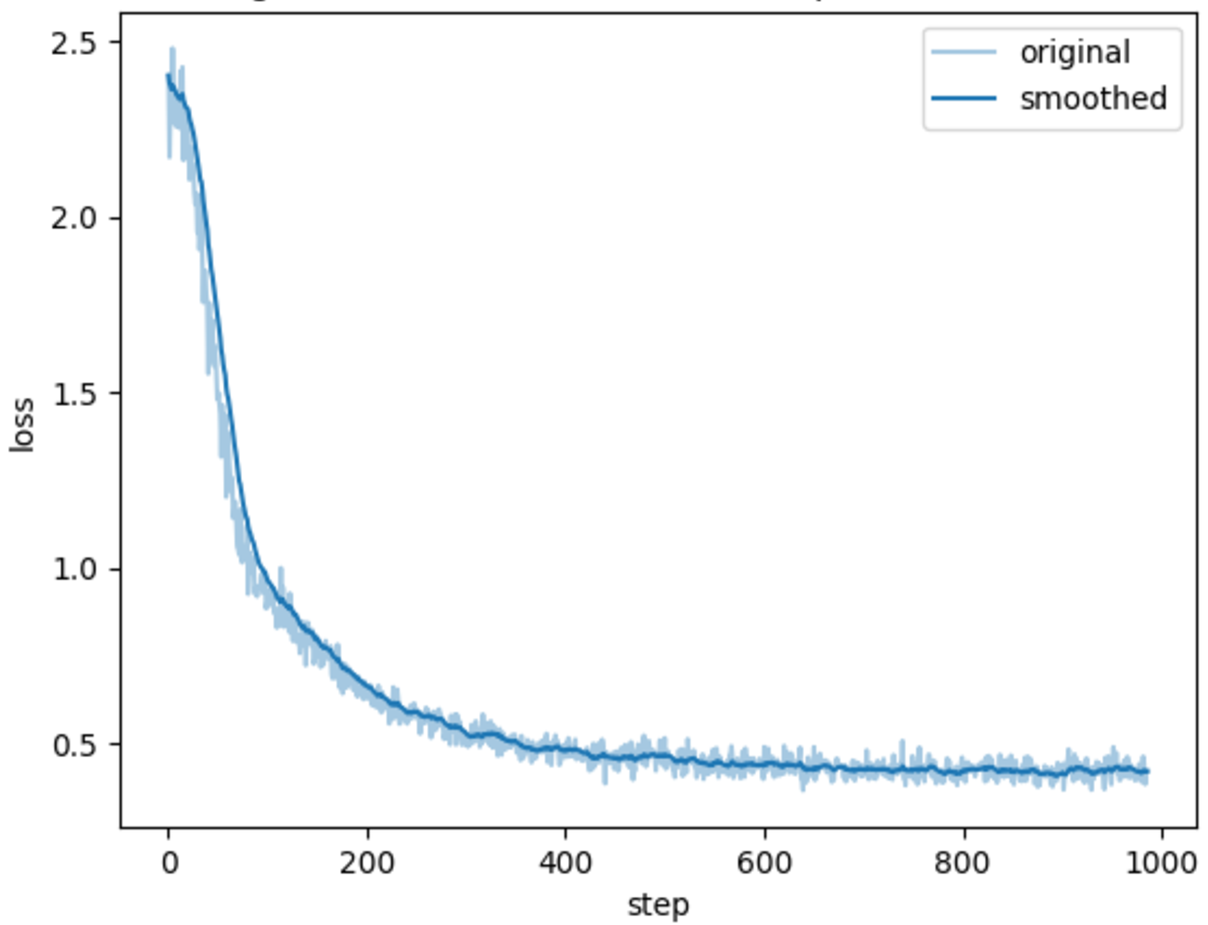
\includegraphics[width=1\linewidth]{Figures/loss.pdf}
    \caption{The training curve.}
\label{fig: training curve}
\end{figure}

\section{Dataset Details}
\textbf{Training Data}

The raw training data in TimeToolBench is collected and organized in ReAct-style format. The characteristic of ReAct-style data is that the structure of reasoning is clear, and the steps always follow the established order of Thought-Action-Observation. We first show a simple example as follows:
\begin{tcolorbox}[
  colback=white,
  colframe=black!50,
  boxrule=0.3mm,
  width=\columnwidth,
  rounded corners,
  title=A ReAct-style Example,
  fonttitle=\bfseries,
  left=2mm, right=2mm, top=2mm, bottom=2mm
]
\textbf{Query}:\\
Here is the time series. Please analyze its pattern.\\

\textbf{Thought}:\\
The most important patterns are trend and seasonality. I will detect them separately.\\

\textbf{Action}:\\
tool: [trend\_classifier]\\

\textbf{Observation}:\\
tool: [trend\_classifier]\\
output: The time series shows up trend ...\\

\textbf{Thought}:\\
I will detect the seasonality next step. \\

\textbf{Action}:\\
tool: [seasonality\_detector]\\

\textbf{Observation}:\\
tool: [seasonality\_detector]\\
The most clear period seems to be 24 ... \\

\textbf{Final Answer}:\\
The patterns are ...
\end{tcolorbox}

During the training process, we hope the overall logic of the context will be preserved. However, this format does not seem suitable for supervised fine-tuning LLMs using the question-answering paradigm. 

To handle this problem, we choose to use the most-liked sharegpt format in LLaMA-Factory. And the above-mentioned example can be organized as multi-turn conversations. Note that the human and observation should appear in odd positions, while gpt and function should appear in even positions. The gpt and function will be learned by the model.

\begin{tcolorbox}[
  colback=white,
  colframe=black!50,
  boxrule=0.3mm,
  width=\columnwidth,
  rounded corners,
  title=sharegpt format,
  fonttitle=\bfseries,
  left=2mm, right=2mm, top=2mm, bottom=2mm
]
\textbf{from human}:\\
Here is the time series. Please analyze its pattern.\\

\textbf{from gpt}:\\
The most important patterns are trend and seasonality. I will detect them separately.\\

\textbf{from human}:\\
(continue)\\

\textbf{from function\_call}:\\
tool: [trend\_classifier]\\

\textbf{from observation}:\\
tool: [trend\_classifier]\\
output: The time series shows up trend ...\\

\textbf{from gpt}:\\
I will detect the seasonality next step. \\

\textbf{from human}:\\
(continue)\\

\textbf{from function\_call}:\\
tool: [seasonality\_detector]\\

\textbf{from observation}:\\
tool: [seasonality\_detector]\\
The most clear period seems to be 24 ... \\

\textbf{from gpt}:\\
The patterns are ...
\end{tcolorbox}



\textbf{Benchmarks}

MTBench is a large-scale multimodal benchmark designed to evaluate the capacity of Large Language Models (LLMs) to integrate and reason across paired time-series and textual data, addressing a critical gap in measuring cross-modal understanding. Spanning the finance and weather domains, the benchmark aligns numerical data—such as historical stock prices and weather records—with corresponding narratives like financial news and storm reports to simulate complex real-world analysis. Unlike traditional benchmarks that focus on isolated modalities or simple prediction, MTBench challenges models with a suite of reasoning-intensive tasks, including time-series forecasting, technical indicator prediction, semantic trend analysis, and news-driven question answering. 

Time-MQA is a unified framework designed to enable multi-task question answering for time series through context enhancement, moving beyond the traditional focus on single numerical tasks. At its core lies the TSQA dataset, a large-scale collection of approximately 200,000 question-answer pairs spanning 12 diverse domains, including healthcare, finance, energy, and traffic. Time-MQA integrates five major categories of tasks—forecasting, imputation, anomaly detection, classification, and open-ended reasoning—into a single question-answering paradigm, allowing users to interact with data via natural language queries supported by textual context. 

In this work, we evaluate on most tasks in MTBench, and choose the subset of TimeMQA, classify them into four categories. The purpose is to ensure that the benchmark datasets do not overlap with TimeToolBench and to evaluate as many types of tasks as possible.

\section{Further Related Work}
Besides Time Series Reasoning, conventional research focuses on Time Series Analysis~\citep{wu2025unlocking,qiu2025comprehensive}, which holds a position of paramount importance across a diverse range of fields, including the economy~\citep{qiu2025easytime,qiu2025multi}, transportation~\citep{wu2024fully}, health \citep{lu2023tf,lu2024mace,lu2025towards}, weather \citep{li2025set,yang2024wcdt,zhou2025reagent}, and energy \citep{sun2025hierarchical}. It encompasses a multitude of critical tasks, such as forecasting, which includes deterministic forecasting~\citep{wu2025srsnet,qiu2025duet,qiu2025dag}, irregular forecasting~\citep{liu2026apn,liu2025astgi}, probabilistic forecasting~\citep{wu2025k2vae,wu2025aurora}, anomaly detection~\citep{zhang2025encode,qiu2025tab,wu2024catch}, classification~\citep{liu2023itransformer,AimTS}, imputation~\citep{wu2022timesnet,gao2025ssdts}, and others~\citep{qiu2025DBLoss,AutoCTS++}. 

Researchers also make efforts to construct time series foundation models to support zero-shot analytical tasks like forecasting~\citep{wang2025lightgts,wu2025flame}, anomaly detection~\citep{units,shentu2024towards}, and classification~\citep{AimTS}. In this work, we adopt them as strong out-of-the-box tools, endowing TimeART the numerical capability.

\section{Details of Tools}
\label{app: tool}

\textbf{Numerical Operators}

\noindent-- \texttt{series\_info}. (). Retrieves basic metadata of the time series, including sequence length (T), number of channels (C), and missing value statistics.

\noindent-- \texttt{datapoint\_value}. (\texttt{index\_or\_timestamp}). Returns the specific values of all channels at a given time index or timestamp.

\noindent-- \texttt{summary\_stats}. (\texttt{start}, \texttt{end}, \texttt{stat}). Calculates a specific statistic (mean, sum, max, min, std) for all channels over a defined index range [start, end).

\noindent-- \texttt{return\_calc}. (\texttt{t1},\texttt{t2}, \texttt{kind}). Computes the percentage return (``pct'') or absolute difference (``diff'') between two specific time indices.

\noindent-- \texttt{autocorr}. (\texttt{lag}). Computes the autocorrelation coefficient for each channel at a specified time lag to measure self-similarity.

\noindent-- \texttt{rolling\_stat}. (\texttt{stat}, \texttt{window}, \texttt{step}). Computes rolling statistics (mean, sum, max, min, std) using a sliding window across the time series.

\noindent-- \texttt{quantile\_value}. (\texttt{q}). Calculates the empirical value at a specific quantile level (between 0 and 1) for each channel (e.g., q=0.5 for median).

\noindent-- \texttt{volatility}. (\texttt{window}). Computes rolling volatility (calculated as the standard deviation of first differences) over a specified window size.

\textbf{Pattern Detector}

\noindent-- \texttt{trend\_classifier}. (\texttt{window}). Classifies trends in time series as ``up'', ``down'', or ``flat''; supports global analysis or window-based segment analysis.

\noindent-- \texttt{seasonality\_detector}. (\texttt{max\_period}). Detects periodic patterns and returns estimated period with seasonality strength (``strong'' or ``weak'').

\noindent-- \texttt{change\_point\_detector}. (\texttt{penalty\_or\_n\_cp}).  Detects structural breaks (change points) in mean or variance and returns the indices of these changes.

\noindent-- \texttt{noise\_profile}. (\texttt{window}). Labels noise type (e.g., ``white'', ``red'') based on autocorrelation tests; performed globally or over a specific window.

\noindent-- \texttt{stationarity\_test}. (\texttt{test}). Tests stationarity using Augmented Dickey-Fuller or KPSS methods; returns status (``stationary''/``nonstationary'') and test statistics.

\noindent-- \texttt{spike\_detector}. (\texttt{threshold}, \texttt{min\_sep}). Detects and locates spikes or dips in the series based on amplitude threshold and minimum separation.

\textbf{Correlation Analyzer}

\noindent-- \texttt{channel\_correlation}. (\texttt{channel\_1}, \texttt{channel\_2}, \texttt{lag}, \texttt{method}). Calculates correlation (``Pearson''/``Spearman'') between two channels with an optional time lag.

\noindent-- \texttt{cross\_correlation}. (\texttt{channel\_1}, \texttt{channel\_2}, \texttt{max\_lag}). Computes cross-correlation across multiple lags to find the optimal time alignment between two channels.

\noindent-- \texttt{dtw\_distance}. (\texttt{channel\_1}, \texttt{channel\_2}, \texttt{distance\_metric}). Measures similarity between two channels using Dynamic Time Warping (DTW); returns distance where lower values indicate greater similarity.

\noindent-- \texttt{shape\_similarity}. (\texttt{channel\_1}, \texttt{channel\_2}, \texttt{norm}). Measures shape similarity between two channels using normalized correlation, invariant to amplitude scaling.

\noindent-- \texttt{granger\_causality}. (\texttt{cause\_channel}, \texttt{effect\_channel}, \texttt{max\_lag}). Tests if one channel statistically predicts another (Granger causality) within a specified maximum lag.

\textbf{Forecasting and Anomaly Detection}

\noindent-- \texttt{anomaly\_detection}. (\texttt{anomaly\_threshold}). Detects anomalies in multivariate time series using the state-of-the-art zero-shot detector DADA~\citep{shentu2024towards} based on reconstruction error (MSE); selects the most significant anomalies by interpreting the threshold as a top percentage (if 0-1) or a specific count (if $\ge$ 1).

\noindent-- \texttt{forecaster}. (\texttt{forecast\_horizon}). Generates forecasts for multivariate time series using the state-of-the-art zero-shot forecaster LightGTS~\citep{wang2025lightgts}; returns predicted values for all channels.

\clearpage
\section{Prompt Templates}
\label{app: prompt}

\begin{tcolorbox}[
  colback=white,
  colframe=black!50,
  boxrule=0.3mm,
  width=\columnwidth,
  rounded corners,
  title=Prompt 1: Making the self-reflections in Stage 3,
  fonttitle=\bfseries,
  left=2mm, right=2mm, top=2mm, bottom=2mm
]

You will be presented with a situation where you need to choose between multiple possible actions.
Your task is to analyze the situation and provide reasoning about why we decide to take the expert action.

\begin{itemize}[leftmargin=1em,labelsep=0.6em,itemsep=0.4ex,topsep=0.5ex]
  \item \textbf{Situation Description ($\mathcal{S}_k$):} \{\texttt{Situation Description}\}
  \item \textbf{Expert Action ($\mathrm{A}_k$):} \{\texttt{Expert Action}\}
  \item \textbf{Expected Outcome ($\mathrm{O}_k$):} \{\texttt{Future State of Expert Action}\}
  \item \textbf{Alternative Actions:}
    \begin{enumerate}[leftmargin=1em,labelsep=0.6em,itemsep=0.4ex,topsep=0.5ex]
      \item Action $\mathrm{A}_k^1$: \{\texttt{Alt Action 1}\}, resulting state $\mathrm{O}_k^1$: \{\texttt{State 1}\}
      \item Action $\mathrm{A}_k^2$: \{\texttt{Alt Action 2}\}, resulting state $\mathrm{O}_k^2$: \{\texttt{State 2}\}
      \item \dots
    \end{enumerate}
\end{itemize}

Provide a detailed self-reflection as an \emph{internal monologue} that demonstrates your reasoning process for the current situation.
Your monologue should:

\begin{enumerate}[leftmargin=2em,labelsep=0.6em,itemsep=0.4ex,topsep=0.5ex]
  \item Analyze the situation and the goal.
  \item Compare the possible actions, explaining why each may be less optimal.
  \item Justify why the expert action is most suitable, grounded in the expected outcome.
  \item Highlight any relevant clues, constraints, or consequences from the situation.
\end{enumerate}

\textbf{Guidelines:}
\begin{itemize}[leftmargin=1em,labelsep=0.6em,itemsep=0.4ex,topsep=0.5ex]
  \item Stay strictly within the provided information.
  \item Avoid meta-commentary about being an AI.
  \item Use natural, step-by-step reasoning.
  \item Focus on logical decision-making.
\end{itemize}

\textbf{Output:} Directly write the self-reflection monologue, no extra headings, disclaimers, or external notes.


\end{tcolorbox}

\begin{tcolorbox}[
  colback=white,
  colframe=black!50,
  boxrule=0.3mm,
  width=\columnwidth,
  rounded corners,
  title=Prompt 2: Collecting the TimeToolBench,
  fonttitle=\bfseries,
  left=2mm, right=2mm, top=2mm, bottom=2mm
]

You are an intelligent Time Series Reasoner capable of performing time series analysis by invoking appropriate tools step by step. \\
\begin{enumerate}[leftmargin=1em,labelsep=0.6em,itemsep=0.4ex,topsep=0.5ex]
  \item Given time series data, a question, and the known answer, reconstruct the intermediate reasoning steps.
  \item You should understand the time series and use the tools to enhance your confidence. You shouldn't completely rely on the results from tools.
  \item You should call a tool at least once to help answer the question. More tool calls are encouraged.
  \item You should think step by step in ReAct-style, output a structured reasoning trajectory that leads to the final answer.
\end{enumerate}
You have access to the following tools: \{tools\}
The only tools you may use are: \{tool\_names\}. \\
"Begin!"\\

The question is: \{input\}
\end{tcolorbox}

\begin{tcolorbox}[
  colback=white,
  colframe=black!50,
  boxrule=0.3mm,
  width=\columnwidth,
  rounded corners,
  title=Prompt 3: Evaluation,
  fonttitle=\bfseries,
  left=2mm, right=2mm, top=2mm, bottom=2mm
]

You are an intelligent Time Series Reasoner capable of performing time series analysis by invoking appropriate tools step by step.\\
\begin{enumerate}[leftmargin=1em,labelsep=0.6em,itemsep=0.4ex,topsep=0.5ex]
  \item You should first understand the question and analyze whether it is necessary to invoke the tool. If not, you can directly give the final answer.
  \item If tools are needed, you can utilize them to help answer the question. Multiple tool calls are encouraged. 
  \item You should think step by step in ReAct-style, output a structured reasoning trajectory that leads to the final answer.
\end{enumerate}
You have access to the following tools: \{tools\}
The only tools you may use are: \{tool\_names\}. \\
"Begin!"\\

The question is: \{input\}
\end{tcolorbox}


\clearpage
\section{Case Study}
\label{app: timetoolbench}

\begin{tcolorbox}[
  colback=white,
  colframe=black!50,
  boxrule=0.3mm,
  width=\textwidth,
  rounded corners,
  title=Sample 1: Anomaly Detection,
  fonttitle=\bfseries,
  left=2mm, right=2mm, top=2mm, bottom=2mm
]

\textbf{Query}:\\
Which value is likely an outlier or anomaly in the dataset [0.06, 0.11, 0.13, 0.14, 0.12, 0.13, 0.15, 0.14, 0.15, \textcolor{red}{0.51}, 0.16, 0.13, 0.12, 0.14, 0.11, 0.10, 0.09, 0.08, 0.07, 0.06]? \\ A) 0.51 B) 0.15 C) 0.14 D) 0.09, \\

\textbf{Thought}:\\
To identify the outlier or anomaly in the dataset, I can use the [anomaly\_detector] tool, which detects anomalies based on reconstruction error. This will help confirm which value is most likely an anomaly.\\

\textbf{Action}:\\
tool: [anomaly\_detector], tool\_input: \{"anomaly\_threshold": 1\}\\

\textbf{Observation}: \\
tool: [anomaly\_detector], 
\\
output: anomaly\_scores: [9.589107503416017e-05, 0.001930518657900393, 0.000164090160978958, 0.0014878634829074144, 0.012693900614976883, 0.021373838186264038, 0.022725816816091537, 0.03277913108468056, 0.05729445442557335, \textcolor{red}{0.1406012624502182}, 3.538517034940014e-09, 0.00018555686983745545, 2.8186357667436823e-05, 2.174061464188526e-08, 4.634935066860635e-06, 0.00020597095135599375, 3.8789648897363804e-06, 0.0008871419704519212, 0.0001234006485901773, 0.0007429602555930614] \\

\textbf{Final Answer}: \\
A) 0.51
\end{tcolorbox}

\begin{tcolorbox}[
  colback=white,
  colframe=black!50,
  boxrule=0.3mm,
  width=\textwidth,
  rounded corners,
  title=Sample 2: Statistical Analysis,
  fonttitle=\bfseries,
  left=2mm, right=2mm, top=2mm, bottom=2mm
]
\textbf{Query}:\\
Calculate and interpret the 3-point moving average of the following sequence [4875.91, 4871.64, 4875.75, 4879.98, 4878.27, 4880.68]. \\

\textbf{Thought}:\\
I need to compute the 3-point moving average for the given sequence. This can be done using the [rolling\_stat] tool with a window size of 3 and the "mean" statistic.\\

\textbf{Action}:\\
tool: [rolling\_stat], tool\_input: \{"stat": "mean", "window": 3, "step": 1\}\\

\textbf{Observation}: \\
tool: [rolling\_stat], 
\\
output: \{"statistic": "mean", "window\_size": 3, "step\_size": 1, "rolling\_results": \{"channel\_0": [\{"window\_start": 0, "window\_end": 3, "mean": 4874.433333333333\}, \{"window\_start": 1, "window\_end": 4, "mean": 4875.79\}, \{"window\_start": 2, "window\_end": 5, "mean": 4878.0\}, \{"window\_start": 3, "window\_end": 6, "mean": 4879.643333333333
\}]\}\}"\} \\

\textbf{Final Answer}: \\
The 3-point moving averages are approximately [4874.43, 4875.79, 4878.00, 4879.64], indicating an upward trend in the sequence.
\end{tcolorbox}

\clearpage
\begin{tcolorbox}[
  colback=white,
  colframe=black!50,
  boxrule=0.3mm,
  width=\textwidth,
  rounded corners,
  title=Sample 3: Compound task,
  fonttitle=\bfseries,
  left=2mm, right=2mm, top=2mm, bottom=2mm
]
\textbf{Query}:\\
Your task is to analyze the past 14 days's of temperature trend and predict the temperature trend for the next 3 days'. The input time series represents temperature readings from 2021-08-19 00:00:00 to 2021-09-01 23:00:00, with a granularity of hourly. Every 24 temperature readings represent a full day from 00:00 to 23:00. The input temperature readings are: [23.3, 22.567, 21.833, 21.1, 20.733, 20.367, 20.0, 20.0, 20.0, 20.0, 20.0, $\cdots$, 19.8, 19.6, 19.4, 19.233, 19.067, 18.9, 18.9, 18.9, 18.9, 19.067, 19.233, 19.4, 19.233, 19.067, 18.9, 19.067, 19.233, 19.4, 19.4, 19.4]. The following events were reported: Flash Flood, Heavy Rain. These occurred near station USW00094823, approximately 23.0844 km away, between 2021-09-01 00:00:00 and 2021-09-01 13:19:00. $\cdots$ Based on the information you received, predict the temperature trend for the next 3 days. Calculate the mean temperature of the last 24-hour period (i.e., the most recent day in the input) and compare it with the mean temperature of the first predicted day. If the difference is greater or equal than 0.5, classify the trend as 'increasing'. If the difference is less or equal than -0.5, classify the trend as 'decreasing'. Otherwise, classify it as 'stable'.\\

\textbf{Thought}:\\
I need to forecast the next 3 days of temperature and compute the mean of the last day in the input and the first predicted day to determine the trend.\\

\textbf{Action}:\\
tool: [forecaster], tool\_input: \{"forecast\_horizon": 72\} \\

\textbf{Observation}: \\
tool: [forecaster], 
\\
output: forecasts: \{'channel\_0': [23.591698, 22.918169, 22.337996, 21.434757, 21.20016, 21.091335, 20.976793, 20.903154, 20.723076, 20.79474, 20.872782, 20.757236, 20.866882, 21.556917, 22.472641, 23.420639, 24.036705, 24.799648, 25.457306, 25.679733, 25.808376, 26.042328, 25.737324, 25.422695, 23.985361, 23.52016, 22.932299, 22.15012, 21.787104, 21.76454, 21.582138, 21.461386, 21.27549, 21.25565, 21.36626, 21.097694, 21.083847, 21.87988, 22.717966, 23.65874, 24.145344, 24.658247, 25.030067, 25.2354]\} \\

\textbf{Thought}: \\
I need to calculate the mean temperature of the last 24-hour period in the input data and the mean of the first 24 predicted values, then compare them to determine the trend. \\

\textbf{Action}: \\
tool: [summary\_stats], tool\_input: \{"start": 312, "end": 336, "stat": "mean"\} \\

\textbf{Observation}:\\
tool: [summary\_stats],\\
output: \{"range": \{"start": 312, "end": 336\}, "statistic": "mean", "results": \{"channel\_0": 19.3875\}\}"\} \\

\textbf{Thought}: \\
I need to calculate the mean of the first 24 predicted values (first predicted day) to compare with the last 24-hour mean. \\

\textbf{Action}: \\
tool: [summary\_stats], tool\_input: \{"start": 0, "end": 24, "stat": "mean"\} \\

\textbf{Observation}:\\
tool: [summary\_stats],\\
output: \{"range": \{"start": 0, "end": 24\}, "statistic": "mean", "results": \{"channel\_0": 22.871\}\}"\} \\

\textbf{Final Answer}:\\
increasing.
\end{tcolorbox}

\clearpage
\begin{tcolorbox}[
  colback=white,
  colframe=black!50,
  boxrule=0.3mm,
  width=\textwidth,
  rounded corners,
  title=Sample 4: Trend Prediction,
  fonttitle=\bfseries,
  left=2mm, right=2mm, top=2mm, bottom=2mm
]
\textbf{Query}:\\
Based on the data points [0.07, 0.04, 0.03, -0.01, -0.06, -0.1, -0.11, -0.12, -0.14, -0.17, -0.21, -0.24, -0.29, -0.34, -0.41, -0.5, -0.59, -0.69, -0.76, -0.82, -0.85, -0.87, -0.88, -0.85], predict the likely trend for the next few data points. \\

\textbf{Thought}:\\
I should analyze the trend in the given data to predict the likely direction of future data points. Using the [trend\_classifier] tool with a global analysis will help determine the overall trend.\\

\textbf{Action}:\\
tool: [trend\_classifier], tool\_input: \{"window": null\} \\

\textbf{Observation}: \\
tool: [trend\_classifier], 
\\
output: \{"trend\_results": [\{"channel": 0, "trend": "flat", "analysis\_scope": "global"\}]\} \\

\textbf{Thought}: \\
The [trend\_classifier] indicates a "flat" global trend, which seems inconsistent with the visibly decreasing values in the data. To better capture the recent behavior, I should perform a window-based trend analysis on the latter part of the series where the decline is most pronounced.\\

\textbf{Action}: \\
tool: [trend\_classifier], tool\_input: \{"window": 10\} \\

\textbf{Observation}:\\
tool: [trend\_classifier],\\
output: \{"trend\_results": [\{"channel": 0, "trend": "flat", "segment\_start": 0, "segment\_end": 10, "analysis\_scope": "window=10"\}, \{"channel": 0, "trend": "down", "segment\_start": 10, "segment\_end": 20, "analysis\_scope": "window=10"\}, \{"channel": 0, "trend": "flat", "segment\_start": 20, "segment\_end": 24, "analysis\_scope": "window=10"\}]\}"\}\\

\textbf{Final Answer}:\\
The data shows a recent stabilization after a period of decline. The most likely trend for the next few data points is flat or a very gradual decline, as the sharp downward movement has slowed in the latest segment.
\end{tcolorbox}


\clearpage
\begin{tcolorbox}[
  colback=white,
  colframe=black!50,
  boxrule=0.3mm,
  width=\textwidth,
  rounded corners,
  title=Sample 5: Pattern Recognition,
  fonttitle=\bfseries,
  left=2mm, right=2mm, top=2mm, bottom=2mm
]
\textbf{Query}:\\
Analyze which statement is correct about the data [39.66, 39.69, 39.91, 40.69, 38.47, 37.5, 36.28, 34.31, 33.12, 33.06, 33.44, 33.72, 33.62, 32.75, 30.44, 29.66, 29.25, 28.5, 28.94, 31.53, 33.0, 35.16, 37.66, 39.62]. \\
A) The data is stable. B) The data shows a clear increasing trend. C) The data mostly decreases with some increase. \\

\textbf{Thought}:\\
To determine which statement is correct, I need to analyze the trend in the data. I will use the [trend\_classifier] tool to classify the global trend of the time series.\\

\textbf{Action}:\\
tool: [trend\_classifier], tool\_input: \{"window": null\} \\

\textbf{Observation}: \\
tool: [trend\_classifier], 
\\
output: \{"trend\_results": [\{"channel": 0, "trend": "flat", "analysis\_scope": "global"\}]\} \\

\textbf{Thought}: \\
The [trend\_classifier] indicates a "flat" global trend. However, visually inspecting the data reveals a clear pattern: it initially increases slightly, then decreases significantly, and finally increases again toward the end. This suggests the global "flat" label may mask underlying dynamics. To better understand, I should examine the data more closely—perhaps by checking for change points or analyzing segments. \\

\textbf{Action}: \\
tool: [change\_point\_detector], tool\_input: \{    "penalty\_or\_n\_cp": "n\_cp=2"\} \\

\textbf{Observation}:\\
tool: [change\_point\_detector],\\
output: change\_point\_results: \{"channel": 0, "change\_point\_indices": [4, 19, 23]\} \\

\textbf{Final Answer}:\\
C) The data mostly decreases with some increase.
\end{tcolorbox}

\clearpage
\begin{tcolorbox}[
  colback=white,
  colframe=black!50,
  boxrule=0.3mm,
  width=\textwidth,
  rounded corners,
  title=Sample 6: Volatility Evaluation,
  fonttitle=\bfseries,
  left=2mm, right=2mm, top=2mm, bottom=2mm
]
\textbf{Query}:\\
Evaluate the volatility of the data [0.52, 0.51, 0.51, 0.5, 0.49, 0.49, 0.48, 0.48, 0.47, 0.46, 0.46, 0.45, 0.45, 0.44, 0.43, 0.43, 0.42, 0.42, 0.41, 0.41, 0.4, 0.4, 0.39, 0.39]. \\

\textbf{Thought}:\\
I need to compute the rolling volatility (standard deviation of differences) for the provided univariate time series. Since no window size is specified, I will use a reasonable default (e.g., window=5) to capture local variability.\\


\textbf{Action}:\\
tool: [volatility], tool\_input: \{"window": 5\} \\

\textbf{Observation}: \\
tool: [volatility], 
\\
output: \{"window\_size": 5, "volatility\_results": \{"channel\_0": [\{"window\_start": 0, "window\_end": 5, "volatility": 0.00489897948556636\}, \{"window\_start": 1, "window\_end": 6, "volatility": 0.00489897948556636\}, \{"window\_start": 2, "window\_end": 7, "volatility": 0.00489897948556636\}, \{"window\_start": 3, "window\_end": 8, "volatility": 0.00489897948556636\}, \{"window\_start": 4, "window\_end": 9, "volatility": 0.004898979485566351\}, \{"window\_start": 5, "window\_end": 10, "volatility": 0.004898979485566351\} \\


\textbf{Final Answer}:\\
The volatility of the data is consistently low, with a rolling volatility (window size = 5) of approximately 0.0049 across all segments, indicating stable and minimal variability.
\end{tcolorbox}





